\documentclass[graphics]{beamer}

\usepackage{graphicx}
\usepackage{verbatim}
\usepackage{wrapfig}
\useoutertheme{shadow}
%\usecolortheme{orchid}
\usecolortheme{seahorse}
\usepackage{tikzsymbols}
\usepackage{textcomp}
\usepackage{parskip}

% math commands
\newcommand{\be}{\begin{eqnarray}}
\newcommand{\ee}{\end{eqnarray}}
\newcommand{\beq}{\begin{equation}}
\newcommand{\eeq}{\end{equation}}
\def\simless{\mathbin{\lower 3pt\hbox
      {$\rlap{\raise 5pt\hbox{$\char'074$}}\mathchar"7218$}}}
\def\simgreat{\mathbin{\lower 3pt\hbox
      {$\rlap{\raise 5pt\hbox{$\char'076$}}\mathchar"7218$}}} %> or of order

% variables

\def\toonscale{0.45}
\def\mboxy#1{\mbox{\small #1}}


\begin{comment}
\AtBeginSection[]{
  \frame{
    \frametitle{Outline}
    \tableofcontents[currentsection]
  }
}
\end{comment}

\title{Helicity
}
\subtitle{}
\author[U. Pen]{\textcolor{green}{Ue-Li Pen}
\\[8mm] 
}
\date{September 26, 2022}


\begin{document}

\frame{
\begin{picture}(320,250)
\put(-50,0){
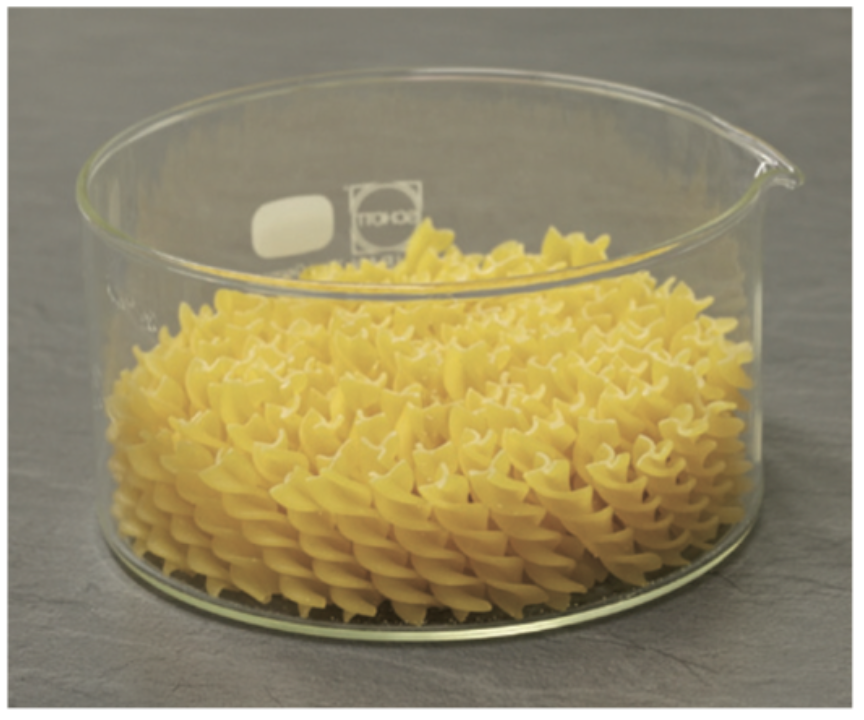
\includegraphics[width=5.5in]{Figures/helicalpasta.png}}
Schaller+12, Nature, 481, 261
\end{picture}
\vspace{-3in}
\titlepage
}

%\section*{Introduction}
\section{Helicity: Kitchen, sun, galaxy and beyond}

\begin{comment}
  \subsection{Outline}

  \frame{
    \frametitle{Outline}
    \tableofcontents
  }
\end{comment}

  \frame{
    \frametitle{Nature}
\vspace{-0.3in}\center{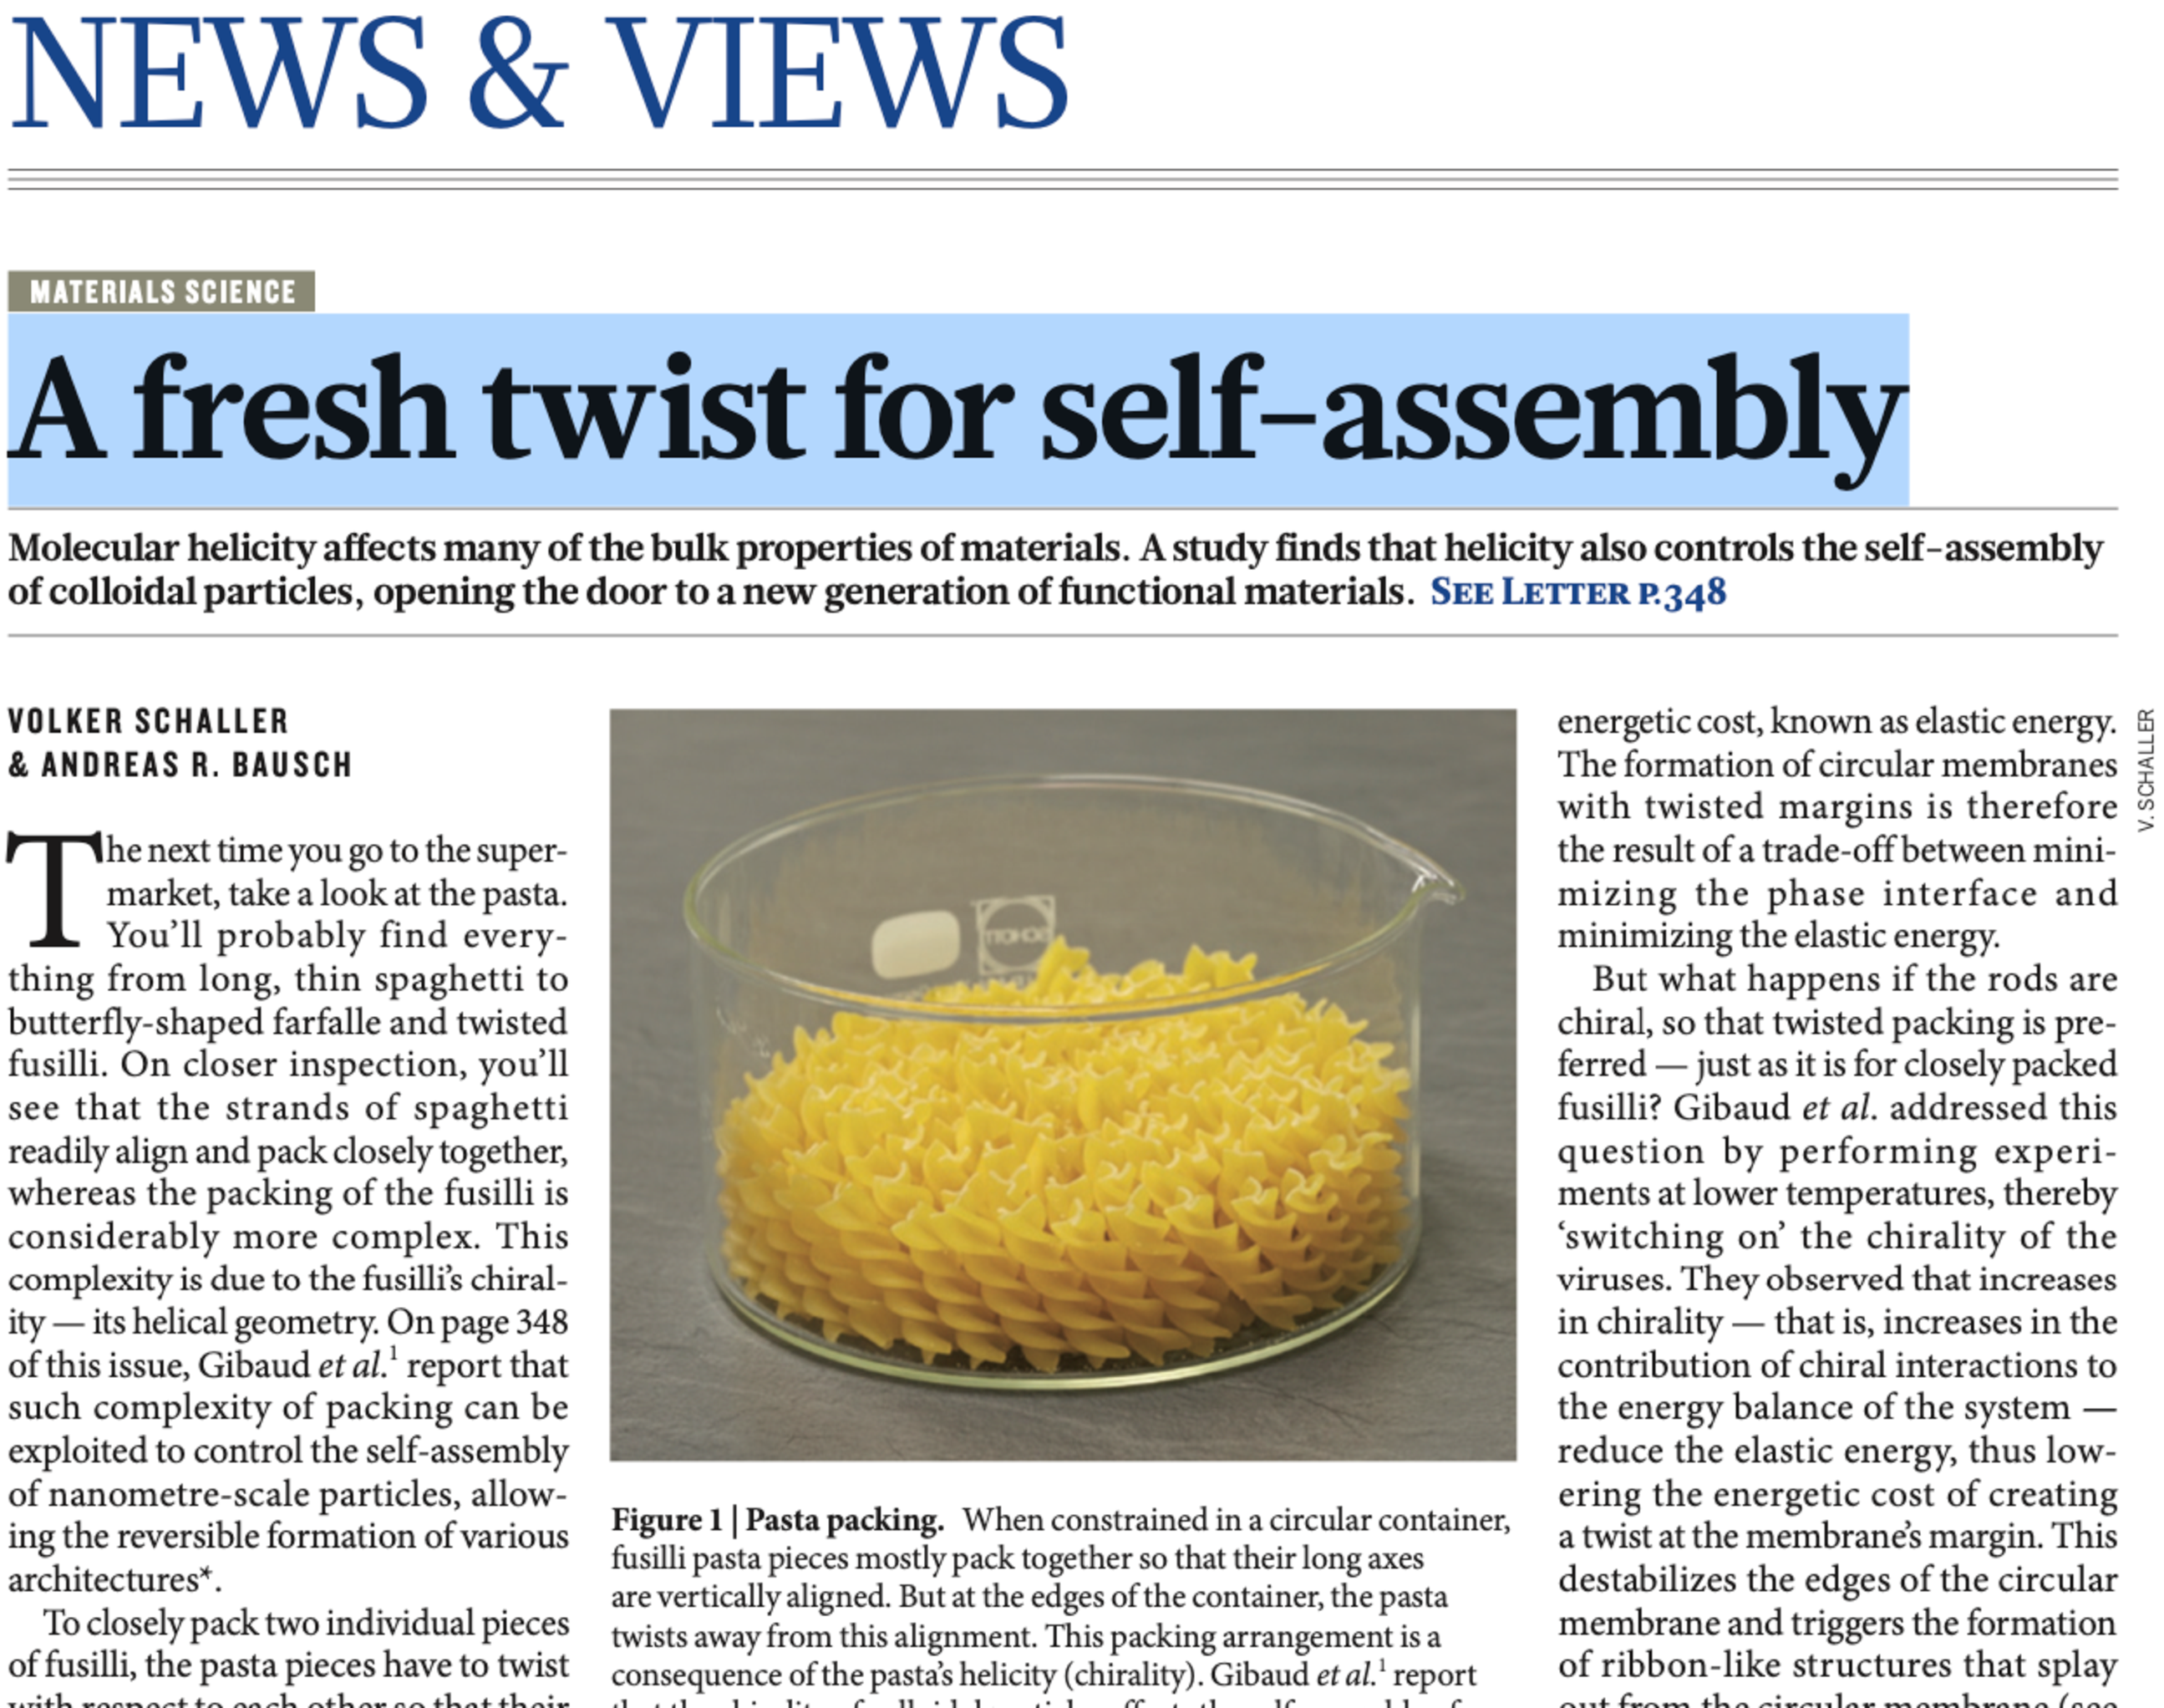
\includegraphics[width=4.0in]{Figures/twist.pdf}}
V Schaller \& A. Bausch 2012, Nature, 481, 268
}
  \frame{
    \frametitle{Pastarimeter}
    %\vspace{-0.3in}
    \center{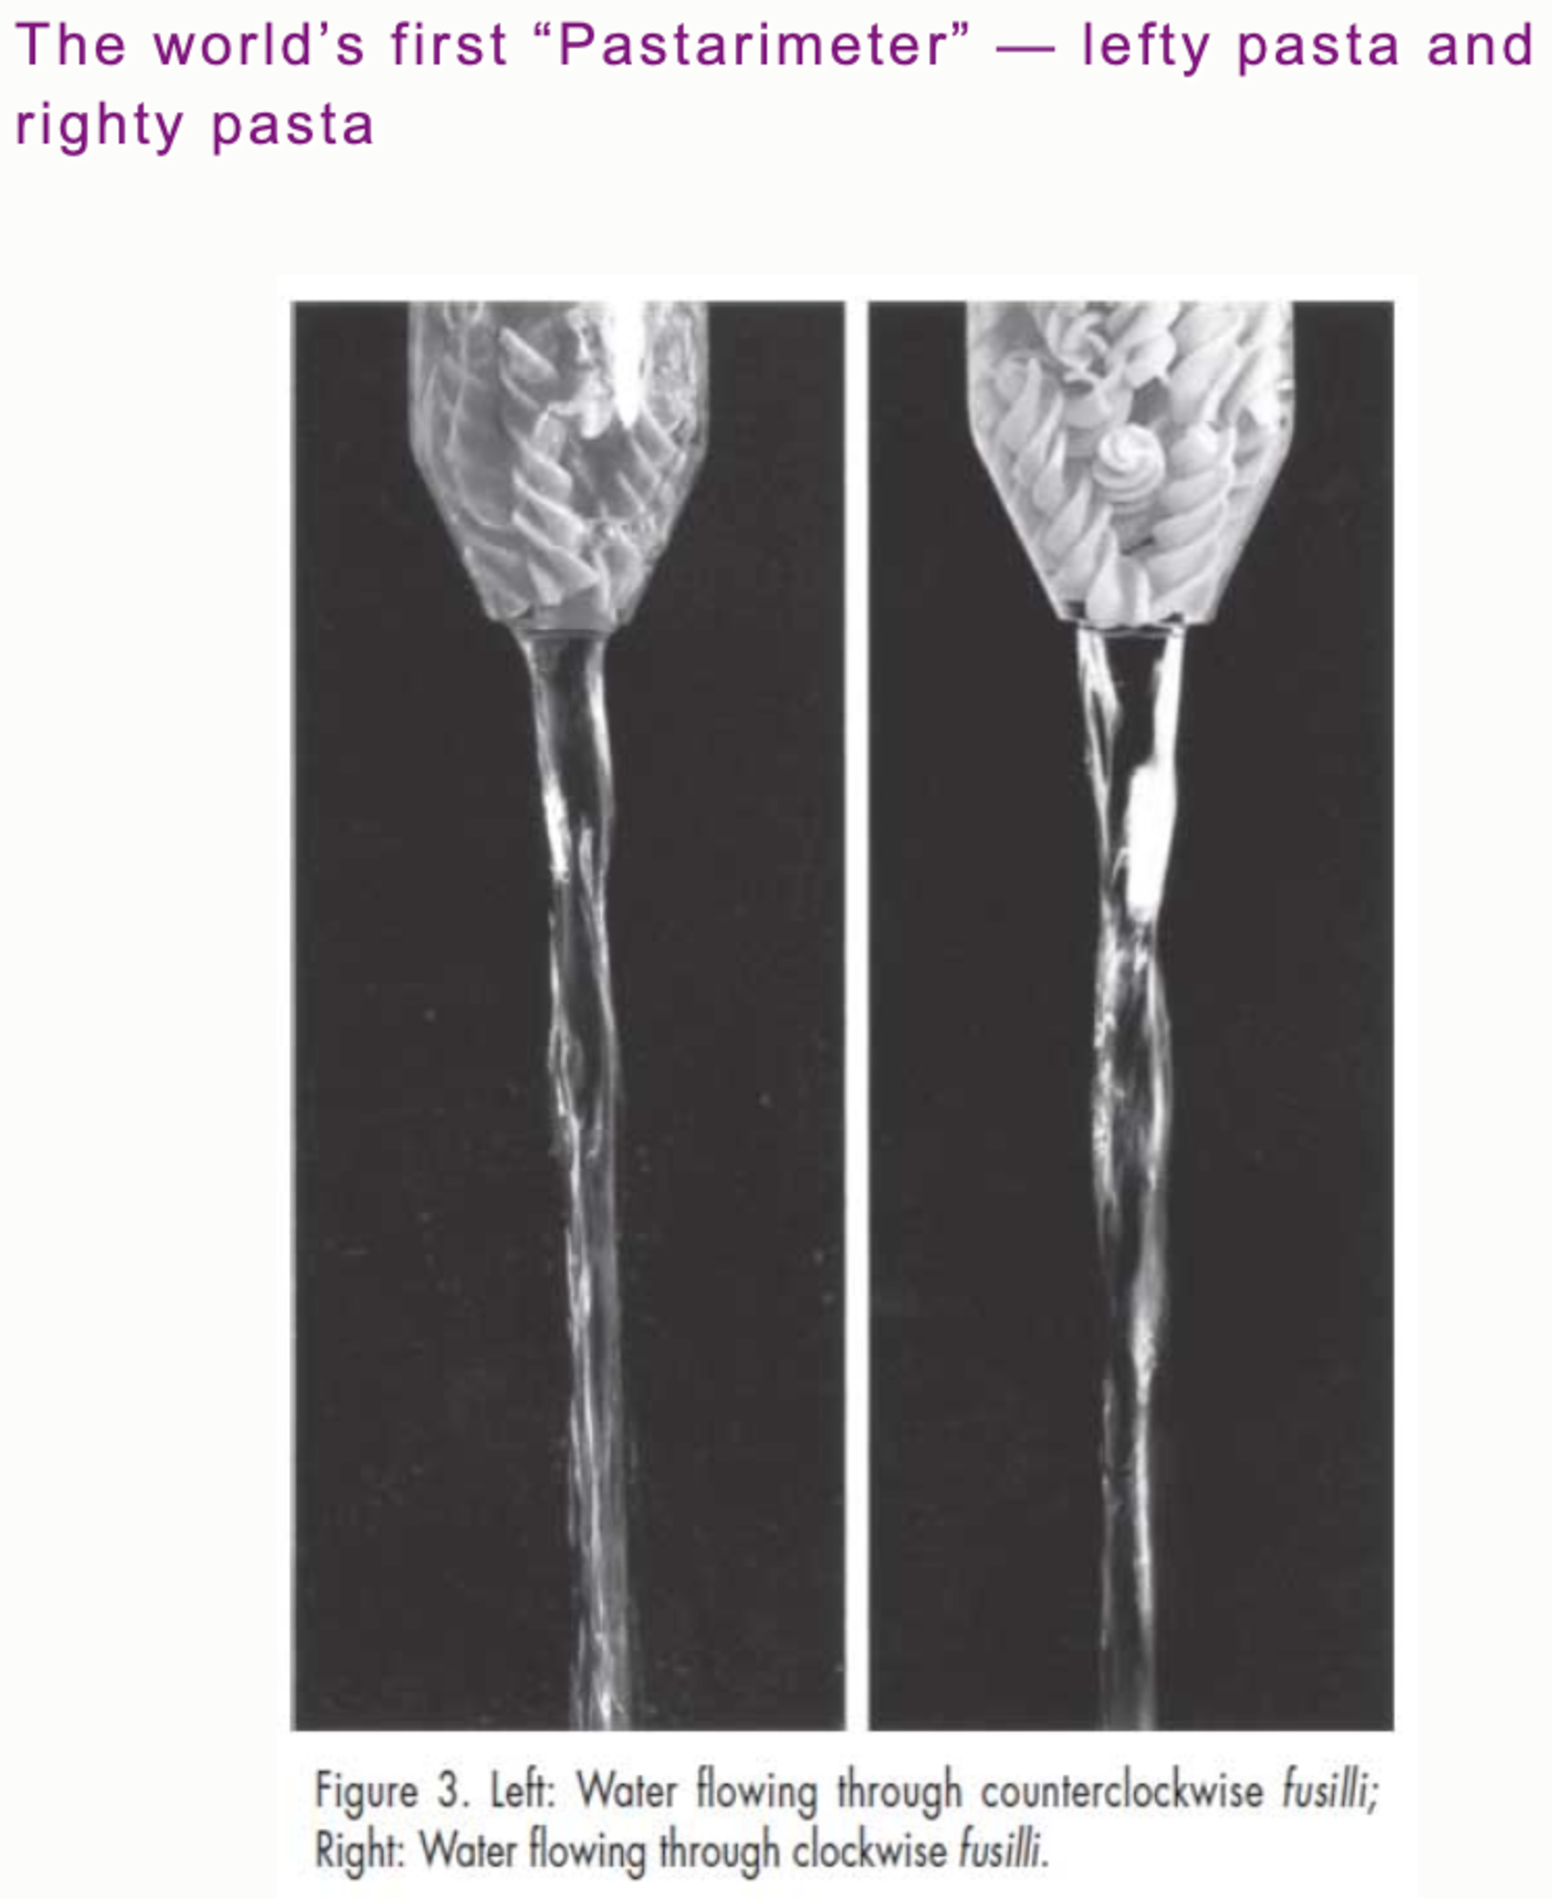
\includegraphics[width=2.5in]{Figures/pastarimeter.pdf}}
{\tiny Saxon et al 2002, J. Chem. Ed, 79, 1214}
}


\end{document}
